\documentclass[
  final,
  babelLanguage=british,
  %desktopVersion,
  %showtrims,
  %overleaf,
]{anecdote}

%\graphicspath{{./assets/photos/300dpi/}}
\graphicspath{{./assets/photos/92dpi/}}

% Page size: 135mm x 120mm
% Body text: 11 / 13.6 pt

\usepackage{local}

%% Details of the book
%% ===================

\title{Allowing Intuition, Revelation, and Insight}
\subtitle{}
\author{Ajahn Vajiro}
\publisher{Publicações Sumedhārāma}
\date{2023-02-13}
\editionInfo{\textit{First edition}, 2023}
\ISBN{978-989-8994-47-9}

% === Metadata ===

\hypersetup{
  pdftitle={\thetitle},
  pdfauthor={\theauthor},
  pdfcopyright={Copyright (C) 2023, \thePublisher},
  pdfsubject={},
  pdfkeywords={},
  pdflicenseurl={https://creativecommons.org/licenses/by-nc-nd/4.0/},
  pdfcontacturl={},
  pdflang={en},
}

%% === Load further packages ===

%% === Hyphenation exceptions and corrections ===

\hyphenation{London}

\begin{document}

\frontmatter

\ifdesktopversion
\desktopCover{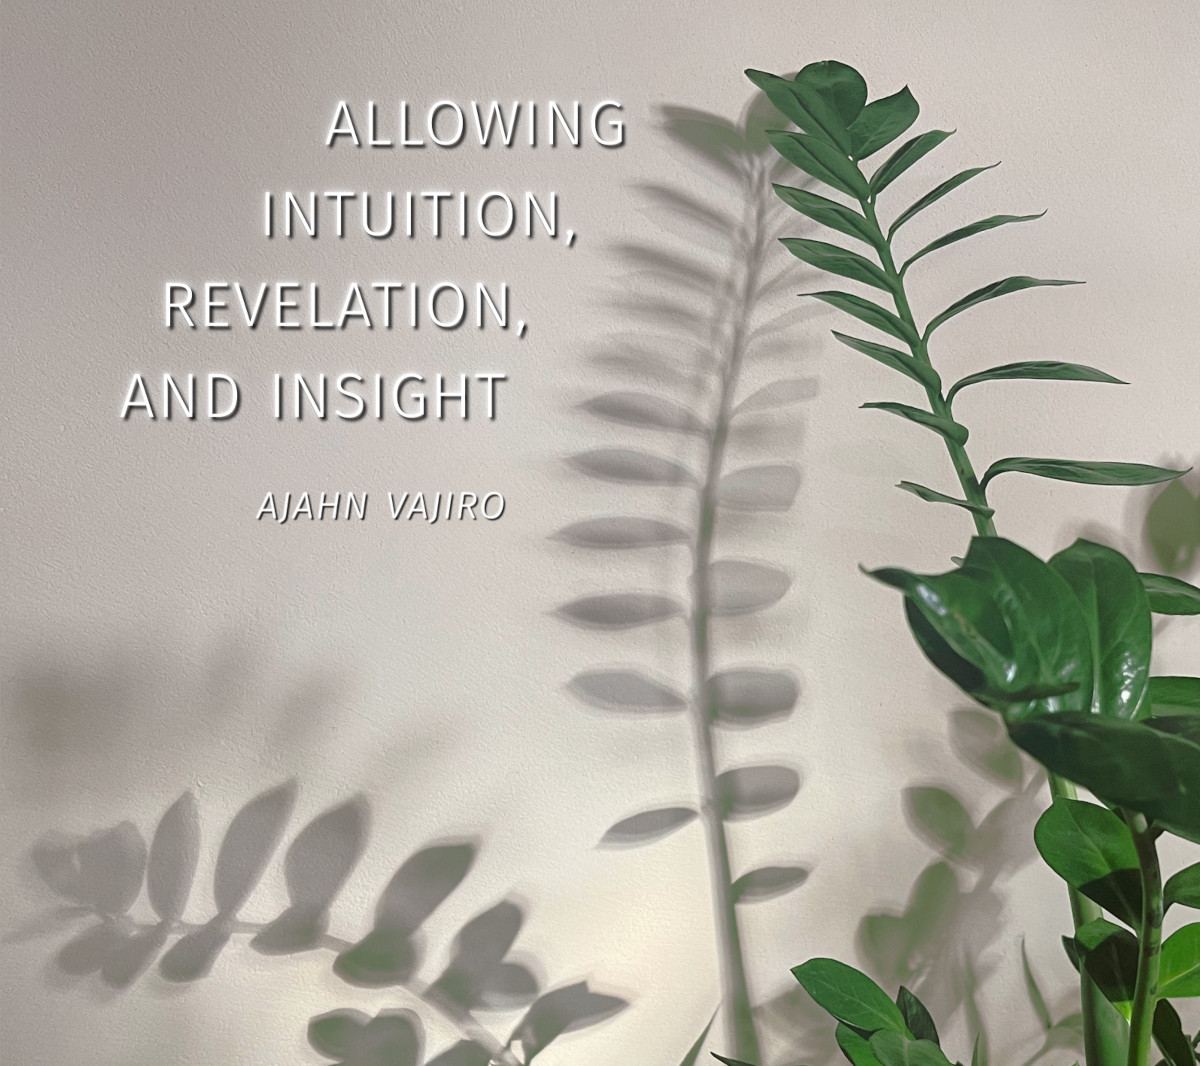
\includegraphics[height=\paperheight]{./desktop-cover.jpg}}
\fi

\cleartorecto
\thispagestyle{empty}
\vspace*{5em}

{\centering

\settowidth{\titleLength}{%
  {\fontsize{13}{13}\chapterTitleFont\scshape\MakeLowercase{\thetitle}}%
}

{\fontsize{13}{13}\chapterTitleFont\scshape\MakeLowercase{\thetitle}}\\[0.3\baselineskip]
\setlength{\xheight}{\heightof{X}}
\raisebox{0.5\xheight}{\color[gray]{0.4}\rule{\titleLength}{0.25pt}}\\[0.3\baselineskip]

\vfill

{\fontsize{10}{10}\chapterTitleFont\selectfont \theauthor}

\vspace*{5em}

}



\cleartoverso
\thispagestyle{empty}

{\copyrightsize
\centering
\setlength{\parindent}{0pt}%
\setlength{\parskip}{0.8\baselineskip}%

\thetitle\\
by \theauthor

Published by \thePublisher

ISBN \theISBN

Copyright \copyright\ \thePublisher\ 2023

This book is available for free download at\\
\href{https://sumedharama.pt}{www.sumedharama.pt}

\vfill

{\footnotesize

This work is licensed under a Creative Commons\\
Attribution-NonCommercial-NoDerivatives 4.0 International~License.

Produced with the \LaTeX\ typesetting system,\\ set in Gentium and Fira~Sans.

\theEditionInfo

}}


% \input{./manuscript/tex/dedication.tex}

% \cleartorecto
% \tableofcontents*

% \input{./manuscript/tex/foreword.tex}

% Page 1 is the first page of the first chapter.
\mainmatter

\chapter{Allowing Intuition, Revelation, and Insight}

{\centering
\begin{minipage}{0.8\linewidth}%
\centering\itshape
This booklet is an adaptation of a Zoom session offered by Ajahn~Vajiro
for the Theosophical Society in America on the 8th~August~2022.
\end{minipage}
\par}


\bigskip

\emph{Ajahn Vajiro:} Welcome everybody. As we gather together and settle, I can
see bouncing people settling into their positions of `I'm going to be mindful
now.' But just remember, and recollect -- as I often do -- that life wishes
itself well, wishes the best for itself.

It may not know what is the best, or it may not have the capacity to find the
best -- but inherently, life strives for the optimum state. It wishes itself
well. Of course, when human beings wish themselves well, they can be very
confused about what's best for them. On an occasion like this where
investigation and a sense of interest are encouraged, it's helpful to remember
why we're doing this. I hope you're not doing this to torture yourself! I hope
you're not doing this to argue with others. If you are, remember that those
are confused ways of trying to wish yourself well, pause, and allow yourself to
be in touch with the sense, the visceral experience, that `this being wishes
itself well'.

The highest happiness and the most complete wellness for human beings is a
happiness independent of conditions -- a happiness that is not reliant on any
condition internal or external. That's the highest. Ajahn Buddhadāsa -- a famous
Thai monk whose name means `servant' (or `slave') to the Buddha -- said that if
human beings work well, they're `happiness creators.' That's a very worthwhile
aspiration to be in touch with.

Anyway \ldots{} this workshop is about allowing intuition, revelation and
insight, and offers some reflections on the nature of thought. And I will begin
by setting down the paradigms, the perspectives, the ways of assuming which are
labelled `right,' and which are wise.

The Eightfold Path begins with \emph{sammā-diṭṭhi} (right view) -- the premise
for us, all ordinary people, that there is giving, offering and sacrifice; there
are results from actions which bring happiness, and results from actions which
bring more pain; there is this world and there are other worlds (ways of
experiencing existence) which are different, which we do not know directly, there are beings which sponaneously arise; and
we have or have had parents (we have received parenting); and there are people, contemplatives and people who
have practised themselves, who can describe and explain these matters through
their own insight.

So there are people with whom it is helpful and skillful to associate, and those
with whom it is not. These are assumptions we can practise that are in tune with
truth. There are assumptions we can hold or practise that are not, and will
bring more pain and confusion for ourselves and others.

So what are we going to practise? And do we know what we are unconsciously
practising?

The second Path factor is \emph{sammā-saṅkappa} -- sometimes translated as `right
thought' -- but in perhaps a more heartfelt way means `right resolve'.

We can choose. And the `right resolve' is `\emph{sammā}', which means `in
accordance with Truth'. By this, I mean `right' as `in tune with' Truth. And I
will, at some point, be giving a working definition of Truth (`Truth' is one
one-word translation of Dhamma). Dhamma is considered precious or
safe. Dhamma is one refuge of the three: the Buddha, the Dhamma,
and the Sangha. Sammā-saṅkappa is thought or resolve that's in accordance with
Dhamma. We can choose and practise creating resolutions or thoughts in tune with Truth.

The description of it is interesting because, as you probably have recognised, a
lot of Buddhism appears negative, and that's because it's easier to notice what
you have stopped yourself from doing, rather than to notice what you are doing. The
resolve that is right is the resolve to renounce, or not indulge; to not to be
cruel or exploit; and to not harm. So, if you find yourself going in those
directions, then those are the practices that are not going to be in tune with
the Dhamma, not in tune with the Truth. And we can notice the space and ease
inherent in a life of renunciation, of a lack of cruelty, and a lack of harm.

To practise feeling and experiencing the neutral is a way to gain a perspective on the spacious and silent. Because the neutral is
something that is easily and often overlooked. And one neutral experience that
we often overlook is incredibly important. That is, this strange rhythm that we
live with twenty-four hours a day: that of breathing in and breathing out. It's
often overlooked, and that's a neutral experience and a thing that is important --
because if we are not doing it, we are in trouble! So for the first phase of
this time together we'll give some time to practising awareness of the neutral,
through careful, kind attention with breathing in and breathing out.

\section{Guided Meditation}

So, now, take up whatever posture you wish -- standing, walking, sitting or
lying down. For most of you, this is probably going to be sitting. A suggestion
that I give is that the posture be something that feels released. That is, we
may feel we have to hold a posture, but the suggestion I like to offer is one of
release.

Be alert and upright, with the eyes open or closed; then receiving an in-breath
\ldots{} and releasing an out-breath \ldots{} Accept the rhythm of the breath
with the gift of attention that is without expectation, regret, or fear \ldots{}

Knowing if the breath is long or short, in or out \ldots{} be this knowing
\ldots{} give life to life \ldots{} without regret or worry or hope or fear
\ldots{}

Allow the attention and the experience to be fully released. Sense the calming
of the body as the whole experience is received and released in the gift of
attention \ldots{} allowing a sense of gentle happiness, to be recognised,
revealed, realised. \ldots{}

Allow the patterns and the rhythms of the heart to also be revealed \ldots{} and
in that revealing, allow calm \ldots{} as the heart is naturally revealed, allow it to lift,
allow the breath to be given out \ldots{} released very softly. Hold the breath
out for a moment, and then sip the breath back in as it's received \ldots{}

Sustain this \ldots{} collecting \ldots{} recollecting \ldots{} sustaining attention.  The heart gathered in this way allows the
shifting, changing experience to be noticed in its natural uncertainty and so not taken so seriously, -- so personally -- and it's allowed to be as it is, and allowed
to end \ldots{} And the ending of things is noticed in this space and this time
\ldots{} the ending of things \ldots{} breath is like this \ldots{} life is like
this \ldots{} now and here \ldots{}

This is a way of allowing space and time, now and here, for intuition,
revelation and insight.

\bigskip

{\centering
\textit{(End of Guided Meditation)}
\par}

\bigskip

There is a human capacity to direct thought and to consciously direct volition
or intention. The volition or intention in the Buddha's teaching is based on the
right view: that there are skilful thoughts and actions that give rise to
skilful results, and there are unskilful ones that do the opposite. Volition or
intention is a cause. There are causes and conditions; when the causes and
conditions for something to be are there, it will be there and when the causes
and conditions for something are not there, it will not be there. Simple as that.

\enlargethispage*{\baselineskip}

Just hearing that much was enough for the Buddha's wisest disciple to gain an
initial understanding. That understanding or realisation forms the initial
premise of the Eightfold Path, that of `right view'. This view proposes that in
the doing of good and wholesome and generous things, there will be good results.
This theme runs through all factors of the Eightfold Path; all factors of the
path are a prescription for the cure for the unnecessary stresses and strains of
the human condition. The Buddha's teachings start with what we can
all relate to: the human condition of irritation, of stresses and strains, and,
discord and disease, and, separation and conflict. The Eightfold Path or Way
offers a practice to mitigate or remove the causes for extra and unnecessary
additions to the stresses and strains. The teachings continue to offer
us guidance on how to relate to the human condition in a way that makes it
noble and worthwhile.

The bit that I want to get to is right view, which offers helpful perspectives,
assumptions, and a paradigm. I like to amplify the idea of `view' -- because
\emph{diṭṭhi} includes how we look at things, and the way we approach things; it
is active. Take, for example, the perspective that we've come from somewhere.
That reminds us that somebody has looked after us at the beginning of our life.
So, in some way or another, the average human being has received kindness. We've
been parented. If a human being is not parented, it dies. So, if you're alive,
you've been parented.

And that's a good thing to base one's perspectives on.

Furthermore, there are things that we don't understand -- states and causes and
conditions that we don't have a clue about. That's useful to recollect, because
if we assume we know everything, and understand everything, then we're going to
fall into the trap of thinking that we never ever make mistakes. And only very
stupid people assume that they never make mistakes.

Another level of stupidity is not to learn from our mistakes. If we are a bit
clever, we learn from our own mistakes. And if we are cleverer still, we try to
learn from other people's mistakes -- that's called `educating ourselves'. So,
the assumption that we don't know everything is helpful; recognising that is a
faculty: the knowing that we don't know.

Humans have the faculty of knowing that they don't know. And then there can be
the realisation that there could be some way of learning. And 
finally there is the faculty of faith that there could be somebody through whom we can learn. These realisations form the
basis and a starting point for wisdom. Based on this wisdom, we can practice resolutions and thoughts
that are beneficial and wholesome give consequent results. Thoughts, -- formed
deliberate intentions, -- that are not skilful produce results that are like the heavy
wheel of the loaded cart pulled by an ox, those which are skilful give results as light as a
shadow.

So we can resolve to renounce or not indulge, to not to be cruel or
exploit, and to not harm, remembering that indulging is a type of self-harming.
Directly resolving to harm, to be cruel, or to exploit others immediately and directly desensitise us.
Indulgence over-stretches or overwhelms the senses, desensitising them, and
resolving to harm or be cruel or exploit also desensitise us. Life is
sensitivity and responding to sensitivity. Life is precious.

And what I've encouraged in the first little meditation exercise was to
breathe through the whole of this. To know whether you are breathing in or
breathing out is always a good touchstone. So, if you find yourself
discombobulated or confused, then you can know whether you're breathing in or
breathing out. And while breathing in or breathing out, you can know whether
your breath is long or short. This is always possible, whatever you're doing.
Through the continuity of that attention and that knowing, your life will be
transformed. That's a promise. Because what will come from that is an interest
in sustaining attention over the whole breath, the whole of the body breathing
-- the whole experience of this important aspect of life.

How does the whole body breathe? As long as this thing is alive, it's going to
be doing this: inhale and exhale -- that's how it is, its basic rhythm. You
can't control this -- there has to be both. How you are with it is very
revealing. It reveals all sorts of moods and tensions. And you can play with it.
Try breathing so that breathing out with your belly's going in, pause the out-breath end. Then
softly bring the breath in by releasing the abdomen. Do that for a
few minutes and see what happens. Then play with a long breath or a short
breath. Figure out what effect that has, and what the interest in that is, and
then see how the habits of the mind reveal themselves.

Getting used to noticing something neutral like that will allow you to notice
what's important that is not usually noticed, not usually received or given
attention.

What's important is where thinking stops. To notice that is useful, because our
assumption is that life is all about thinking. But there is that which is not
thinking, and there is space around thought. Thought begins and ends. So, you
notice what you don't usually notice. Silence. Space. What is not thinking?

Maybe I should now give a definition of `truth.' In Buddhism, this is called
`Dhamma'. Dhamma is translated in quite a few ways. My teacher often translates
it as `The Way It Is'. It's described in the scriptures as something that is
`revealed by wisdom', `revealed by the supreme teacher, the Buddha.' The truth
is already there -- whether it's realised or not. Truth is something that is
immanent, apparent here and now. Truth is this here and now. It's something that is always this
present time and space. It's also eternal, outside time. The Dhamma is not bound by
space or by time.

Thought is all about time. Thought is about interpretations and simplifications,
and quickly moves through proliferation. It's something bound up in time. The
Dhamma as a precious refuge is not bound up in or by thought; it's outside of
space and time.

And, the truth is always encouraging and inviting investigation. It may not
yet be revealed, but equally it is not hidden. It is beautiful. Knowing
the truth, in the realising of the truth, there's a sense of discovery, of a
beauty that is hidden in plain sight.

Even things that appear somehow disgusting or terrible, in the knowing of those
-- `It's like this' -- then there's the encouragement to investigate, and the
knowing and the realisation: `This is how it worked' \ldots{} `This is what
happened. This is how it is.'

The release or ease that comes with realisation is an aspect of truth. It leads
the mind inwards (or onwards) to a sense of peace and resolution. It is also
humbling. Because the truth is open and realisable by everyone -- by each person for
themselves.

One might hold the idea that everybody finds their own truth. No. People realise
the truth for themselves. But if it's just my truth, then it's different from
your truth, and that's going to lead to conflict. It's not going to be something
beautiful, or attractive, or encouraging investigation. The truth isn't
personal; it's not my truth. The realisation is now and here. And humans have the
capacity for this because they have the capacity to act through body, speech, and
mind by directing and understanding volition, or intentional thought. This is
why the human birth is the most fortunate birth. Other beings do not have the
same capacity for directing intentional volition through thinking.

\enlargethispage{2\baselineskip}

When the heart is free from confusion, greed, and hatred, there's naturally a
sense of gratitude. One wishes suffering for oneself and others to abate. One
can feel this sense of gratitude with every breath: it's not that you have to
focus intensely on breathing -- but to appreciate it. It doesn't need to be held
on to. It's enough just to acknowledge: `Breathing is lovely.' And it's
important to be grateful for gratitude!

\clearpage

\section{Questions and Answers}

\emph{Question:} It is hard to live without any hope or expectation or desires.
However, I can see these hopes and desires are the cause for more suffering. Is
hoping to get recognition a type of greed? Is needing recognition a form of lack
of self-worth?

\emph{Ajahn Vajiro:} I've been mentioning Ajahn Buddhadāsa and his saying that humans,
when they work well, are happiness creators, and saying that we can find
happiness in whatever we're doing. Find happiness in what you're doing. We can do things for their own sake rather than for an end result.
And we can practise contentment as a support of happiness.
One day I was present when he was asked about fear.
Someone asked him something along the lines of, `What can I do to get rid of this fear I usually have?' Ajahn Buddhadāsa didn't
reply directly. So I was interested in that, and I was very surprised when he
responded by asking the questioner, `What do you hope for?' He didn't ask, `Why
are you frightened?'; he asked `What's your hope?' I realised that one cause of fear is hope, and the accompanied
worry that you're not going to get the result that you want.

\enlargethispage{2\baselineskip}

Now it's not that we can't aspire for something or make a resolve. But these
are different from hope. We can begin with a sense of `I can do this. If I
work with this, then this can happen' -- that is based on contentment and builds confidence. But with
hope we're setting ourselves up for fear. If you hope to be famous, then
you're going to be frightened that nobody knows you. If you hope that some
particular person will be your friend or the perfect partner, you're setting
yourself up for feeling rejection. Then you're caught in the worldly winds of
being famous or being ignored or vilified. There are these worldly winds: gain
and loss; fame and disrepute; pleasure and pain; and praise and blame. Those are
the vicissitudes of life. But the happiness that's independent of conditions is
not bound by those. Again, as Ajahn Buddhadāsa said: `Joy at last, to know that
there is no happiness in the world!' If you're looking in the wrong place when
you're looking for happiness, then you're setting yourself up for disappointment
and fear. This is a form of ignorance, and a sense of not having enough is a
kind of greed, or can go the other way into a sense of rejection, anger or
overwhelm.

\bigskip

\emph{Question:} How do I know when I am allowing for intuition, revelation and insight,
rather than navigating this life on self-direction? Like, when is it inspired
rather than manufactured by self?

\emph{Ajahn Vajiro:} Complicated, isn't it? But insights and strong spiritual
experiences can be helpful, even transformative. So, I don't like to put them
down. They can come through a lot of self-effort -- a lot of hammering away at
things. However, this can lead to breakdown and psychosis because the hammering
can be misplaced -- willpower can damage delicate aspects of the psyche. Yet
sometimes there can be great insights. Whether they're true or not goes back to
the definition that I gave: if they bring a sense of resolution, awe, and
humility, they're true.

I find revelation to be experienced something like: `What? I believed that for so long? I didn't see this.' It is accompanied by a sense of calm and lack of conflict.

Remember the marker on the door, where you line up against the door and your
parent draws a little line to see how much you've grown from year to year? The
test of your spiritual progress, I suggest, is like this: how are you with yourself and
other people? How are you in relationship? How you are with other people is a
test. With the people that you know, the ones you don't know very well, those
you dislike in your daily life, is your life a blessing, or a
curse? That's a test, isn't it? Whatever insight you may have, if it
upholds or glorifies self, then it doesn't bring unshakable blessings to your life. One
way of putting it is: `The personality is not enlightened; enlightenment is
about losing the sense of the self-importance of ``I''.'

If you're thinking, `I'm striving for enlightenment', you're going to get
disappointed. Enlightenment is understanding this whole sense of `I', and not
taking it so seriously. Because this `I' is a construct. The basic blockage is:
`I am somebody; I need to do something; and I'm not sure if I can do it, or if
it's the right thing.' That's the basic blockage around which the whole thing
revolves, the complications go round and round. And for other people the complication we put on them: `You are somebody, you need
to do something, and I'm not sure whether you're going to do it.' That sets up
me as being somebody who wants you to do something. See how that complicates our
whole existence. It adds stress to our life, and to those of other people, as we
swirl around in these thought patterns. I'm somebody, I have this history, this social
conditioning, this story, and I need to do something. And of course, I'm not
sure if I can do it, or if it's the right thing. So, Ajahn Vajiro is somebody,
and he needs to tell me what I need to do! And then I'm still not sure whether he is telling me
the right thing or not, or if I can do it.

You're not going to get out of that in that way. Sorry! Because that's the whole
self-view -- along with the clinging around self-view, the search for the
technique or magic formula, and the doubt/confusion about if it will work or if
we can work it -- and there is not a way out of it through more thinking and believing in this.

\enlargethispage{2\baselineskip}

Understanding self-view, and the search for something to do, and the doubt that
maybe this `something' is the `wrong-thing', or maybe I can't do it; this understanding is
said to be more difficult than defeating a thousand warriors in hand-to-hand
combat. It's not easy. And it's not going to be Ajahn Vajiro telling you how to
do it, however strongly you think: `But he must. I've signed up for this. I want
the insight.' What I'm trying to point out is that this sense of self is
bound up in thought. `How do I know whether I'm allowing intuition, revelation,
and insight, rather than navigating this life on self-view? Like when is it inspired,
rather than manufactured by self?' Thoughts like this will just keep spinning, keep
entangling, keep knotting up, heating up, and stressing.

\clearpage

\emph{Question:} Could you please speak a bit about the relationship between
thought/time? Can we have in ourselves a part in time and something out of time
and profound, an absolute truth?

\emph{Ajahn Vajiro:} Thought and time are not so difficult to understand, because a
thought has a beginning and an end, and time is created in thought. Through
participating in these online meetings, we recognise that we live in our own
time and space. We are not all in Illinois. In our own time and space we relate to the time and space of others.

Thinking gives us a sense of time and space, so notice what's not thinking \ldots{} 
start with noticing the space between thoughts, when one thought stops
and another begins \ldots{} similar to breathing which has an in and an out.
An in-breath begins and it ends, and an out-breath begins and ends, and there's
a space around. Similarly, a thought begins and ends. And you can stop the
thought; it's not that difficult to do. Notice it and then stop it. Maybe the
habit is to start another thought quite quickly. But with a bit of practice,
it's possible to stop that. You can stop it altogether, of course, when you
absorb into something still. But that might take a bit more effort than most of us are
willing to give. Maybe a shortcut is to notice what's not thinking \ldots{} of
course, the noticing isn't thinking. That which is aware is not thinking, and
that's a gateway. For most of us, that awareness doesn't seem important, so it's
overlooked. But overlooking something that in fact is important is a mistake.

\enlargethispage{\baselineskip}

\bigskip

\emph{Question:} Can you hope without attachment?

\emph{Ajahn Vajiro:} Life is going to seek happiness -- that's the nature of it. It's a
responsive thing. Even amoebas move away from that which is uncomfortable. But
the happiness that's really worthwhile is a happiness independent of conditions.
The difficulty with sensory happiness is that it can't be sustained, because
sensory experience at the five senses is actually an irritation. So, you can't get happiness from
the senses all the time. Also, with the sensitivity that we have, this form of
happiness will always have the background anxiousness that, `If it's happy now, it's
going to go away or end or there will be pain.'

\bigskip

\emph{Question:} Please talk about the role of attachment in happiness.

\emph{Ajahn Vajiro:} You can aspire without attachment. Hope is tied up with
attachment. Aspiring contains contentment and carries the sense: `I can give into this.' And a basis of
release is the sufficiency that comes with that sense of: `I can give.' Hope, on
the other hand, makes and leaves a hole. When I hoped to have the perfect
something, I created this image of something that was going to complete my
world. And then when I got it, of course, all I realised was that it didn't. I
had put energy into the attitude of: `I'll only be complete if I get this.' And
by doing so I created and put energy into feeling incomplete. Then that energy put into the sense of incompleteness had to find something else to project onto,
something else to attach to, be born into. So be careful about hoping for things, and instead
go to the attitude of: `If I do the right things, if I work in the right way,
then I can do this.' This is what I call aspiration, and it offers a direction
that doesn't go to disappointment, and doesn't feed the sense of inadequacy that
comes with, `If I get this, then I'll be happy.'

\bigskip

\emph{Question:} Can you please talk about the understanding of what happiness is, and
the experience of it according to the Buddha? How is joy related to or different
from happiness?

\emph{Ajahn Vajiro:} Yes, this relates to Ajahn Buddhadāsa's phrase, `Joy at last to
know that there is no happiness in the world.' This is not to say there's no
pleasure; rather that no lasting happiness can be found in the pleasures of the world. For
Buddhists, the goal is about freedom from the compulsion that is born of
ignorance -- freedom from the blindness of habit. However, freedom comes with
understanding this stress, and releasing the compulsion to act from it rather
than dwelling in aversion to it. We are encouraged to act in ways that relieve
stress and strain now and in the future. This is compassion, which requires
wisdom, and is the natural expression of a heart free from ignorance. It has
lasting results and also brings about a sense of appreciation and joy in the
presence of goodness. This leads to an acceptance and a serenity that is able to
accept the limitation of this time and this space, and to act without regret or
hope.

These are aspects of what are called the \emph{brahma-vihāras}: loving-kindness,
compassion, joy, and serenity -- \emph{mettā, karuṇā, muditā, upekkhā}. These
are the natural expressions of the heart free from ignorance.

The Buddha expressed and taught the Dhamma -- a way of understanding. He also
taught the Vinaya, which is a way of behaving. He taught both these to relieve
suffering. The basic Vinaya or training for humans is to train to not take life, to not take
what's not given, to not misuse sexuality, to not lie, and to abstain
from alcohol and drugs -- because these impair the power of judgement. A human
society is when people keep the five precepts; basically, human society relies
on that. By and large most humans most of the time don't kill, don't steal, don't misuse their
sexuality, don't lie, and don't get intoxicated. When they do, that's through
confusion. The joy of a heart free from confusion is natural.

\enlargethispage{\baselineskip}

\bigskip

\emph{Question:} So how do I balance trusting myself and my intuition versus getting
carried away by the sense of self? And how do I know when thought is intuitive?

\emph{Ajahn Vajiro:} Often you don't know. But you have some guidelines -- such as the
five precepts. So, if you have the intuition that you will have to kill
somebody, you know that's one that you don't follow. Keep it simple. One of the
most generous things you can do as a human being is to keep the five precepts!

The other way of testing your intuition is to maintain the sense of, `I'm not
sure', so that you're willing to learn from any mistakes you make. Entertain
the possibility that things might be different. Know that you don't know, and
then know what you can know -- this knowingness, now. By all means, have plans,
but know that plans are just plans, and what actually happens is different from
a plan. Know that maps are just maps, and they don't actually correspond to
what's on the ground and the mud beneath your feet. So, keep a sense of humility
with regard to your intuitions, resolve not to harm, exploit or indulge. And with speech \ldots{} practise not lying, gossiping, or using harsh or pointless
speech. In terms of your livelihood, practise according to the Eightfold Path.
Also, try to find good friends that can give you some guidance. However,
remember that in every situation, when you approach it -- you just don't know!

When people ask me `what shall I do?' I can't tell whether they should do this or whether they
should do that. For the most part, all I can say is `I don't know', and `You'll
have to find out.' A commitment is helpful, because it gives you something to
work with; constantly drifting doesn't help. Particularly useful is a commitment
to wishing to learn from experience, and to understand. Thought is always just
thought, and intuition is beyond thought, but sometimes your intuition can just
be a distortion, so don't always trust it. I can't give you clear answers
because how it is will have to be how it is for you.

However, in terms of how to relate in ways that give life nobility and value,
this comes about through the responses that go against the habits of merely seeking
pleasure through the senses, or through power. Yet this is not about completely
denying anything, getting tight and tough, or punishing oneself.

\bigskip

\emph{Question:} What is a relationship to life that is ennobling and worthwhile?

\emph{Ajahn Vajiro:} Well, any sense of existing as a separate entity is going to be
tied up with stresses and strains. And for humans in particular the sense of aging, of breaking down or breaking apart,
 of separation from what is liked and loved, of being disappointed, not getting what one wants and being bothered irritated and annoyed by what is, these are inevitable. Understanding this is ennobling and worthwhile.
The drive for extra stress is compulsion to seek satisfaction from the next thing… and the next… and the next. And the compulsion to get rid of, or away from pain and anguish. The cycle of being pleased with something and then disappointed. 

The experience that is now and here is the limitation that we live with, and
committing to accept and understand this limitation, not to demand that it be otherwise, helps
us to abandon the thirst and compulsion that is the cause of extra suffering.
All this compulsion is born out of ignorance. Because in this moment here there is this. And
it is complete. If it wasn't meant to be this way, it wouldn't be this way.

So having recognized that sense of: `I want it to be different; I want to get
rid of this; I want to get on to the next bit', the noble relationship is to
abandon these compulsions. Because compulsion puts extra stress on the system.
Then one can notice that there is an end to this stress. Making that abandoning of compulsions
into a reality there is a sense of completeness, fulfilment and freedom. This
makes life worthwhile and noble.

\enlargethispage{2\baselineskip}

I'd like to do that. Certainly, that's what encouraged me when I first met
people who were not looking to gain something and not worried about loss; not
worried about praise and blame; not worried about a little bit of pain; not
trying to get pleasure and be famous -- people who weren't living according to
worldly aims and values. This is important: if you're interested in liberation,
don't live according to worldly aims and values. Life is a gift, and our life
depends upon giving.

How often is a simple act of kindness part of your life? It's what allows us to
work well. Then also work on your ways of communicating, because we do feel
separate. And communicating is a way to connect, and skilful communication is and brings blessings.

Practise a livelihood that's not damaging -- something that's not
involved with exploiting animals or other human beings, not involved with
dishonesty, weapons or poisons. 
It may be difficult to practise this because of our social system. For example,
if you're involved in the financial system, it's difficult to get some sort of
livelihood that's completely separate from exploitation and spreading lies. What
I noticed years ago, when looking at advertisements, was that all that the
advertisements are telling us is that, `You are inadequate. If you don't get
this, you won't be happy.' That's encouraging a sense of inadequacy. I never
felt that that was skilful. In fact, it's a very unskilful message to be
spreading around. 

Instead, investigate your life, and notice habits and
behaviours in yourself and others that you feel, `These aren't helpful',
and don't pick them up. That's a useful way to start \ldots{} by not doing
something. It gives you the space to look at what is unskilful in your heart,
and give that up. Then notice what is skilful, and keep that going. Maintaining
what supports and grows goodness and wisdom is right effort, which requires mindfulness.

Mindfulness in itself is just attention. Often, we pay attention because we want to get something in return -- we pay
attention in order to get a result. When you're absorbed into something and
paying full attention to it, it may be incredibly exciting and dangerous, and force
you to pay attention -- that's exciting. But this is not going to lead to
liberation. However, noticing that you can collect, gather, give and sustain full attention is helpful. 

Practice instead giving attention to the body; the responses of the senses;
where things are coming from, and the source of all that; giving attention to the
ways things work in the mind. This will lead to liberation. Giving attention to
the breath, the movement of the body and the nature of the body, knowing and
seeing it for what it is, all of this leads to liberation.

Notice how the heart is in the moment -- whether it's confused, constricted,
open or bright -- where is this coming from? Then notice whatever stops
the continuity of attention: where are the distractions? See them for what they
are, that they begin and end; see what feeds them.

Notice all this as part of a process -- then you can work with it. Notice what
cultivates attachment, and then notice what liberates, and cultivate that
noticing itself: how it arises, how it ends, and what sustains it. Then go back
to noticing the nobility and what works in terms of giving value and worthyness to life, so you keep
returning to the Four Noble Truths. The sustaining of that process is the practice of the
Eightfold Path: right view, right intention, right thought, right action, right
livelihood, right effort, right mindfulness and right concentration. Practise
the Eightfold Path, because that's the only thing that will make life
worthwhile. This gives human existence a blessing; it is the right relationship
to Truth.

\enlargethispage{\baselineskip}

The Eightfold Path leads to happiness independent of conditions. If you're not
asking for conditions to make you happy, you're able to give happiness. If
you're looking outside of the Path for happiness, you're not able to give it --
even if you're looking to make other people happy. If you're looking to see
whether other people are happy or not, you're going to be disappointed, because
your happiness will be dependent upon their response. Find a happiness
independent of conditions through a sense of `This is what I can do. This is
what I can offer', and then you'll be able to offer happiness. Whether people
accept it or not, that's not your business. Even the Buddha couldn't make
anybody enlightened; he could only offer people the opportunity to practise so
that they could realise for themselves.

Right view (\emph{sammā-diṭṭhi}) that leads to liberation is insight
into the Four Noble Truths. In this, the understanding of \emph{dukkha}, the
abandoning of its cause, the realisation of its ending and the practice of the
Path all happens at the same time. The rest of the Path turns according to the
degree to which there's right view. The other factor of the path that has the
Four Noble Truths in it is right mindfulness -- mindfulness in accordance with
truth. What this is about is not taking anything personally. When I said that
the first three fetters are: `I am somebody, I need to do something, and I'm not
sure if I'm doing the right thing or not, or if I can do it or not', that's
taking this whole thing personally. The practice of right mindfulness is: `Oh,
it's like this.' Nothing's personal. It's all just causes and conditions.

Of course, humans are cause creators. But there's more to it. There's the cause
of physical things, how they work. There's the cause of how genetics works.
There's the cause of how the heart can work things. And there's the cause of the
way that \emph{kamma} (that is, intention) works. When the causes and conditions
for something are there, the thing will be there. And when the causes and
conditions for the thing are not there, the thing will not be there. That is the
basic teaching of all the Buddhas.

\bigskip

\emph{Question:} What does cultivating the heart mean to you? And how important is it
on the path?

\emph{Ajahn Vajiro:} Yes. Cultivating the heart is the practice of the Path. The sense
of separation that comes from me and you, the sense of wanting to manipulate
what's outside of me, that's a cause of \emph{dukkha}, stress. The result of the
heart going out into all this is that more or extra stress is generated. I mean that
taking it personally, as in: `This is something that I have to do something
about. This is for me, and I've taken ownership of it' this `ownership' adds
stress. Because then this mass of stress is \emph{my} self. Cultivating the
heart is about not taking experience personally. It's leaving things like this
alone. This is very important. Now, if I say, `It's important to me', then I'm
going to try to attach to the Path. Then it's going to be me that will have the
insights and me that's going to be practising the Path. But it's not like that.
Instead, what can be done is to notice this sense of separation and to let that
be.

What we can do is keep the attention inwards, so it doesn't go out into wanting
to harm, doesn't go out into wanting to exploit or be cruel, doesn't go out into
wanting to indulge. The attention is kept inwards. Then what comes out is not
going into actions of speech that are harmful, and not going into livelihoods
that are harmful, because there's this sense of containment. That allows the
sense of frustration -- that `I can't do what I want' -- to be transformative.
It brings patient endurance: sustained patience in the moment with things being as they
are. That's the supreme way of transforming the sense of separation -- knowing
that, `However difficult it is, I can bear this in this moment.' Willingness to
practise this comes as you gain confidence, and this can be transformative.
People have transformed their lives by following and committing to a discipline.
A discipline of harmlessness, non-exploiting and non-indulgence transforms the
society one lives in. That's where spiritual progress can be measured: by how
much it transforms the society that you live in. So yes, do cultivate the heart.

\bigskip

\emph{Question:} What is attention, as compared to concentration?

\emph{Ajahn Vajiro:} There are many discussions about what constitutes right
concentration or \emph{sammā-samādhi}. In the scriptures, it is described as the
four \emph{jhānas}. These four \emph{jhānas} are described in the commentaries
in some detail, but are not so completely described in the scriptures. So the
result is that there can be some discussion about \emph{jhāna}. However, to be
brief, practising \emph{jhānas} as described in the commentaries is about
absorbing into something. It's a useful thing to do, but that absorption doesn't
in itself lead to insight. What does lead to insight is sustaining attention, a
heart freed from the hindrances, collected, cool, released, when thought itself
is not believed in. This is a way of talking about \emph{samādhi} that I find
interesting. The topic is worth investigating. I generally don't talk about
concentrating the mind. Instead, I talk about gathering, collecting,
recollecting, clarifying -- words that support a sense of steadying, and
settling and appreciating \ldots{} I feel that such suggestions are more
sustaining.

\bigskip

\emph{Question:} Could you please define the self? Is there a self? Who has
aspirations? Who is helpful? Who is skilful?

\emph{Ajahn Vajiro:} `Who is helpful? Don't Buddhists teach about non-self?' On being
asked a direct question by the wanderer Vacchagotta as to is there a self or not,\footnote{\href{https://suttacentral.net/sn44.10/en/bodhi}{SN 44.10: Ānanda Sutta}} the Buddha remained silent. Well, in terms of experience,
there is this mind, and this body here; and this mind and this body can be
trained. The Buddha's teaching on non-self (\emph{anattā)} is about not taking
this living thing, or even life itself, personally. Form, feeling, perception,
conception, and consciousness do manifest, and these are what we identify with
as `for me' and so `mine' and proliferate into `I' and `My Self'. This is what we take personally. But obviously, these
are not completely controlable. A self, if it's mine, should be completely
controllable, and should be something that's always happy, never disappointing.
Otherwise, it's not worth calling it a `self.' However, anything that is form,
feeling, perception, conception, or consciousness, if claimed as self, if taken
personally, is going to disappoint you -- because none of these are stable.
This sense of self is inherently stressed, dependent on conditions so why take it personally? It's just the way nature works; it belongs to nature; give it back
to where it belongs. Don't claim something as yours that's not yours. Why settle
for second-best, when happiness independent of conditions can be realised?

Now, I'm not saying that the conventional `self' can't have some happiness. Certainly, this
separate entity experience can work well. To the degree that it does
reduce extra suffering for itself and for others, and encourage happiness independent of conditions then that's the degree to which it
is skilful. We'd all like to realise our full potential,
wouldn't we? I can remember at age sixteen thinking `I don't want to waste my
life.' And indeed I have led a privileged life. I'm incredibly grateful for it.

\bigskip

\emph{Question:} Is the Eightfold Path the way to combat the eight worldly winds? And
also, the way to root out greed, hatred and delusion? I think it takes close
monitoring not to react or to say anything unskilful when we are with people who
are speaking unskilfully.

\emph{Ajahn Vajiro:} Yes! That's a reasonable summation. Close monitoring means
mindfulness, attention in the present moment, a sense of being able to give
attention and to receive life. Then, when people are speaking unskilfully to
you, the reaction is noted for what it is. You're not trying to stop the
reaction, but you don't have to add to it, and you don't have to believe it. You
know the old story -- if somebody's shouting and yelling at you, you get angry
with them, but if somebody tells you, `they're crazy, they don't know what
they're doing', your sense of anger disappears. Or if a toddler throws a
tantrum, you don't expect it to do anything else. You don't indulge that
tantrum, but you also don't blame it for throwing a tantrum, because it's a
toddler; it doesn't know why and what it's doing. When you realise that most of
us are confused mentally, physically, and spiritually, then blaming others for
how they are behaving, or blaming ourself for how we are behaving is
unproductive. The best attitude is, `Let's practise and offer what we can.'
Because the human realm is like this! It IS deeply confused. At the moment, it's
great if we can keep it good enough -- but in the end, nature doesn't care,
nature will just run on as nature does.

I'd like to express gratitude to all teachers who's support I've received and I apolgise for any and all mistakes or distortions added through ignorance.
I wish you all the very best, and if there have been any blessings generated
may they be shared with all beings \ldots{} may we all practise the Way and
realise happiness independent of conditions. Thank you!



\newpage\null\thispagestyle{empty}
\clearpage

% \backmatter

\clearpage
\thispagestyle{empty}

{\fontsize{8}{12}\selectfont%
\setlength{\parindent}{0pt}%
\raggedright\label{copyright-details}%
\setlength{\parskip}{5pt}%

{\centering

{\LARGE\ccbyncnd}

This work is licensed under a Creative Commons\\
Attribution-NonCommercial-NoDerivatives 4.0 International~License.

\href{https://creativecommons.org/licenses/by-nc-nd/4.0/}{https://creativecommons.org/licenses/by-nc-nd/4.0/}

}

You are free to:

\begin{packeditemize}
\item Share — copy and redistribute the material in any medium or format
\end{packeditemize}

The licensor cannot revoke these freedoms as long as you follow the license terms.

Under the following terms:

\begin{packeditemize}
\item Attribution — You must give appropriate credit, provide a link to the license, and indicate if changes were made. You may do so in any reasonable manner, but not in any way that suggests the licensor endorses you or your use.
\item NonCommercial — You may not use the material for commercial purposes.
\item NoDerivatives — If you remix, transform, or build upon the material, you may not distribute the modified material.
\end{packeditemize}

No additional restrictions — You may not apply legal terms or technological measures that legally restrict others from doing anything the license permits.

\clearpage
\thispagestyle{empty}

Notices:

You do not have to comply with the license for elements of the material in the public domain or where your use is permitted by an applicable exception or limitation.

No warranties are given. The license may not give you all of the permissions necessary for your intended use. For example, other rights such as publicity, privacy, or moral rights may limit how you use the material.

% TODO confirm this notice with The Publisher

\thePublisher\ asserts its moral right to be identified as the author of this book.

\thePublisher\ requests that you attribute ownership of the work to \thePublisher\ on copying, distribution, display or performance of the work.

}


\emptyUntilEven

\end{document}
